\section{Solving a Real-World Problem Using Reinforcement Learning}
Is to apply reinforcement learning techniques to solve a real-world problem. Students used a publicly available dataset to train an RL agent, evaluated its performance, and optimized it to achieve the best possible outcome.
\newline
The exercise will utilize the Taxi-v3 environment available in the OpenAI Gym repository. This environment simulates a simplified grid world where an agent must pick up and drop off passengers at the correct locations while avoiding walls and other obstacles. We used Dataset/Environment: Taxi-v3 on OpenAI Gym.
\newline
\subsection{Understanding the Environment}
The Taxi-v3 environment from OpenAI Gym is a reinforcement learning (RL) environment. The goal of this environment is to solve tasks using RL algorithms. It uses a state and action space, allowing for experimentation with various RL algorithms, such as Q-learning and Deep Q-Networks (DQN)[21].
\newline
The agent's goal is to pick up and drop off passengers at specific spots on a 5x5 grid. The agent must drive the taxi to pick up a passenger, take them to the right location, and do all of this before time runs out[21].
\newline
\newline
\textbf{Environment Overview}
\newline
\newline 1.State Space: The state is a tuple of:
Ï. The taxi's position on a 5x5 grid.
II. taxi has a passenger. 
III. The destination is 4 possible locations: the four corners of the grid.
\newline
2. Action Space: The taxi has 6 possible actions:
Move north, Move south, Move east, Move west, Pick up a passenger, and Drop off a passenger.
\newline
\begin{figure}[H]  % The 'H' forces LaTeX to place the figure here
    \centering
    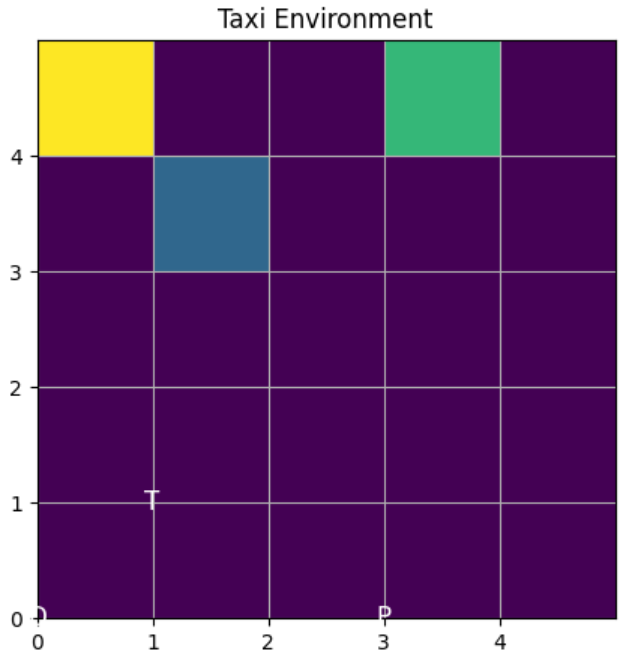
\includegraphics[width=1\linewidth]{figures/Taxi_Environment.PNG}
    \caption{Taxi Environment}
    \label{fig:Taxi Environment}
\end{figure}
3. Rewards: 
A. A positive reward for correctly dropping off a passenger.
B. A negative reward for each illegal move.
\newline
\begin{figure}[H]  % The 'H' forces LaTeX to place the figure here
    \centering
    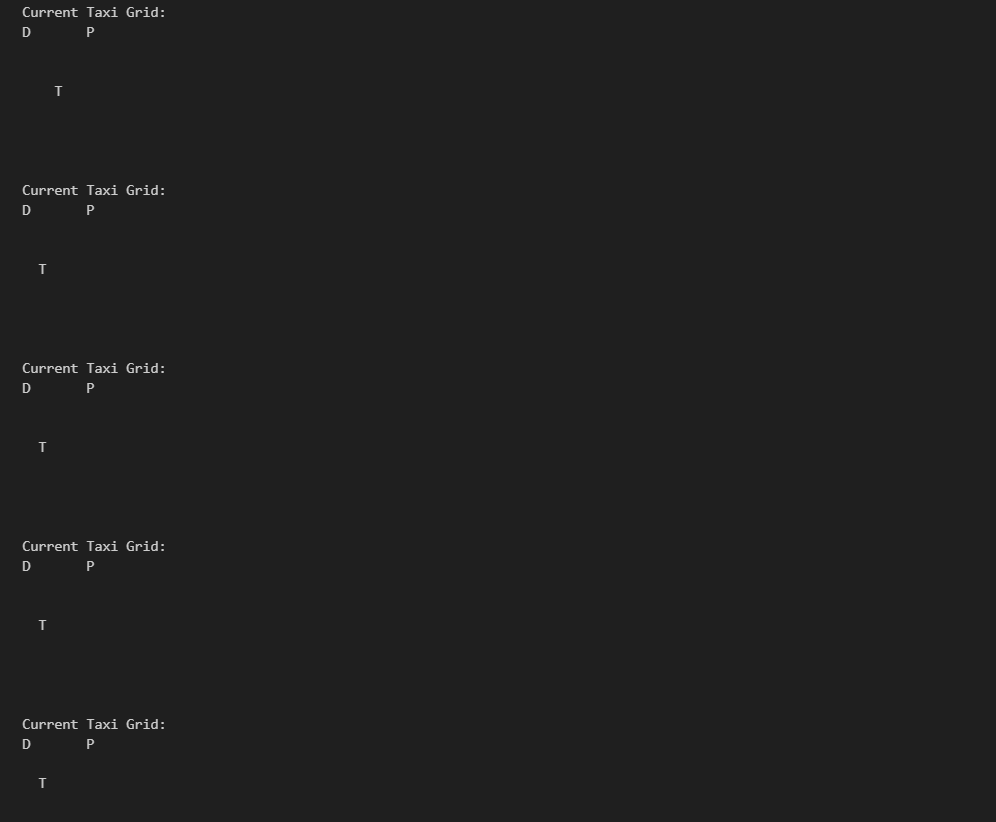
\includegraphics[width=1\linewidth]{figures/Taxi_moves.PNG}
    \caption{Taxi Moves}
    \label{fig:Taxi Moves}
\end{figure}
4. Termination: The episode ends when the passenger is successfully dropped off.
\subsection{Setting Up the RL Agent}
to steps set up the Q-learning Agent in the Taxi Environment we got the throw steps:
\newline
1. Set up the environment: Initialize the Taxi-v3 environment from Gym. In our case, we encountered a problem using Gym, so we used Gymnasium instead.
\newline
2. Initialize Q-table: Create a Q-table state-action value table to store the values of state-action pairs.
\newline 
Set hyperparameters like learning rate, discount factor, and exploration rate. In our case, we used the following hyperparameters:
\begin{itemize}
    \item \texttt{learning\_rate} = 0.8 \quad \# Alpha.
    \item \texttt{discount\_factor} = 0.95 \quad \# Gamma.
    \item \texttt{epsilon} = 1.0 \quad \# Epsilon.
    \item \texttt{epsilon\_min} = 0.01 \quad \# Epsilon minimum.
    \item \texttt{epsilon\_decay} = 0.995 \quad \# Epsilon decay rate.
    \item \texttt{num\_episodes} = 1000 \quad \# Total number of training episodes.    
\end{itemize}
4. Training Loop: In each episode, we reset the environment using reset, and the agent selects an action based on the epsilon policy. This takes that action in the environment, and updates the Q-table using the Q-learning update rule[22],[23].

\begin{itemize}
    \item Initialize environment \(\mathcal{E}\) and agent \(\mathcal{A}\).
    \item For each episode \(e = 1, 2, \dots, E\):
    \begin{itemize}
        \item Reset the environment: \(s_0 = \mathcal{E}.reset()\).
        \item For each time step \(t = 0, 1, 2, \dots, T\):
        \begin{itemize}
            \item Choose action \(a_t = \mathcal{A}(s_t)\) based on current policy.
            \item Execute action \(a_t\) in the environment: \(s_{t+1}, r_t = \mathcal{E}.step(a_t)\).
            \item Update agent's policy\(r_t\) and \(s_{t+1}\).
            \item If the episode ends, break the loop.
        \end{itemize}
    \end{itemize}
\end{itemize}
5. Epsilon greedy policy: The agent selects a random action with probability epsilon. 
6. Evaluation: After training, we evaluate the agent by running a set number of episodes, and then the agent selects the best action according to the trained Q-table.
\subsection{Training the RL Agent: }
In order to train the RL agent on the Taxi-v3 environment, we set up the hyper parameters as follows:
\begin{itemize}
    \item \texttt{learning\_rate} = 0.8 \quad \# Alpha
    \item \texttt{discount\_factor} = 0.95 \quad \# Gamma
    \item \texttt{epsilon} = 0.1 \quad \# Epsilon
    \item \texttt{num\_episodes} = 1000 \quad \# Total number of training episodes
    \item \texttt{max\_steps\_per\_episode} = 100 \quad \# Max steps in an episode
\end{itemize}


\begin{figure}[H]  % The 'H' forces LaTeX to place the figure here
    \centering
    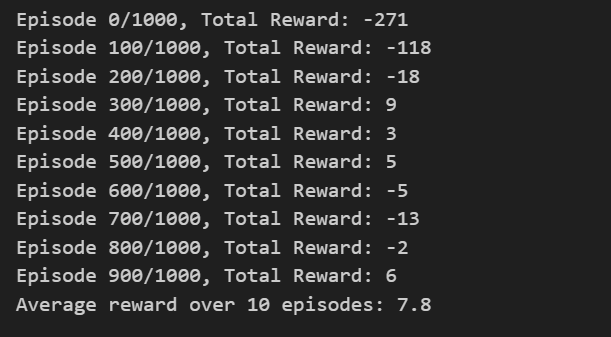
\includegraphics[width=1\linewidth]{figures/Q-Table_Evaluate.PNG}
    \caption{Q-Table Evaluate}
    \label{fig:Q-Table Evaluate}
\end{figure}

\begin{figure}[H]  % The 'H' forces LaTeX to place the figure here
    \centering
    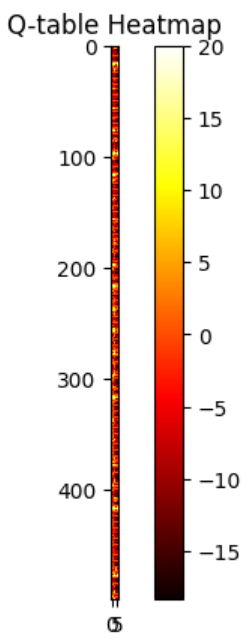
\includegraphics[width=0.5\linewidth, height=0.5\textheight]{figures/Q-Table_HeatMap.PNG}
    \caption{Q-Table Heatmap}
    \label{fig:QTableHeatmap}
\end{figure}

\subsection{Evaluation}
\begin{figure}[H]  % The 'H' forces LaTeX to place the figure here
    \centering
    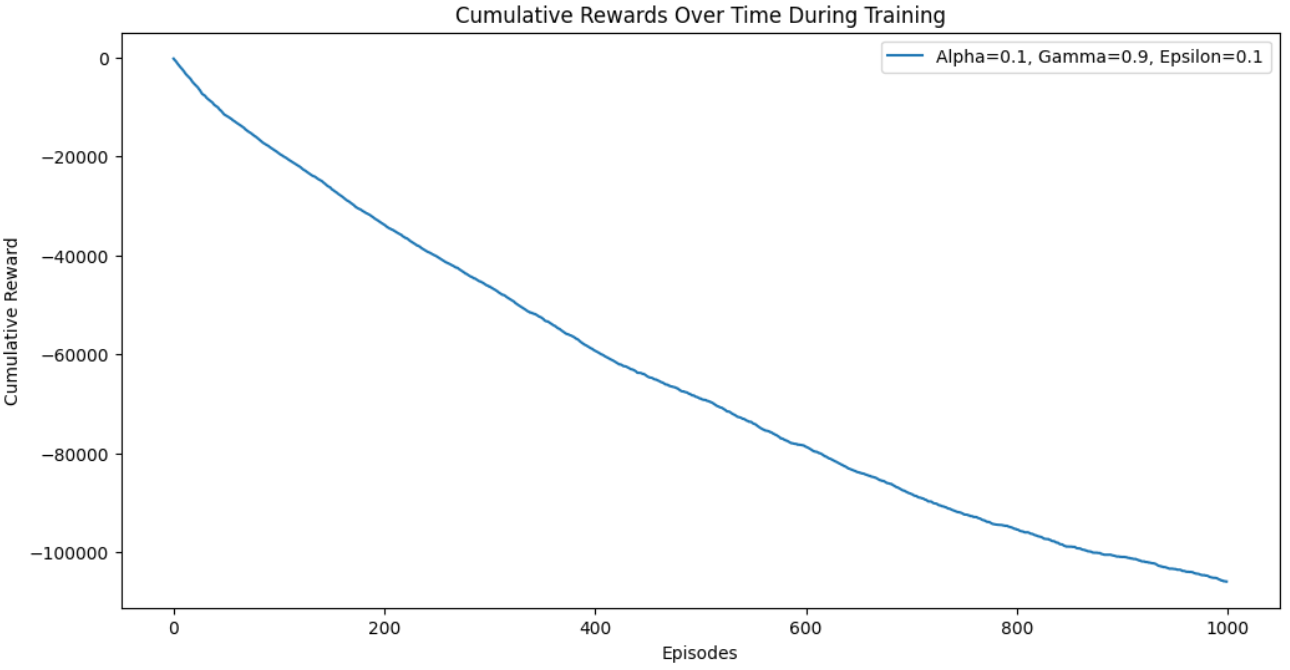
\includegraphics[width=1\linewidth]{figures/Cumulative_Rewards_Over_Time_During_Training.PNG}
    \caption{Cumulative Rewards Over Time During Training}
    \label{fig:Cumulative Rewards Over Time During Training}
\end{figure}







